\documentclass[11pt,a4paper,openany,twoside]{book}
%-------------------------------------宏包引用---------------------------------------------------
\usepackage[paperwidth=155mm,paperheight=230mm,textheight=170mm,textwidth=110mm,left=20mm,right=25mm, top=35mm, bottom=25mm]{geometry}            %定义版面
%--------------------------------------------------------------------------------------
\usepackage{fontspec}
\usepackage{xunicode}
\usepackage{xltxtra}
\usepackage[slantfont,boldfont]{xeCJK}
%--------------------------------------------------------------------------------------
\usepackage[listings,theorems]{tcolorbox}
\usepackage{fancybox}                 % 边框,有阴影,fancybox提供了五种式样\fbox,\shadowbox,\doublebox,\ovalbox,\Ovalbox。
\usepackage{colortbl}                   % 单元格加背景
\usepackage{fancyhdr}                 % 页眉和页脚的相关定义
\usepackage[CJKbookmarks, colorlinks, bookmarksnumbered=true,pdfstartview=FitH,linkcolor=black]{hyperref}   % 书签功能,选项去掉链接红色方框
\usepackage{tabularx}
\usepackage{tcolorbox}
%\usepackage{ctex,ctexcap}

%-----------------------------源代码---------------------------------------------------------
\usepackage{listings}
\usepackage{lineno}

%--------------------线条加粗-------------------
\usepackage{booktabs}
\usepackage{multirow}

%-------------------caption字体----------------
\usepackage[font=footnotesize]{caption}

\usepackage{scrextend}

%--------------------折现图------------------
\usepackage{tikz}
\usepackage{pgfplots}

   %引用宏包所在位置
%-----------------------------------------------------主文档 格式定义---------------------------------
\addtolength{\headsep}{-0.1cm}        %页眉位置
%\addtolength{\footskip}{0.4cm}       %页脚位置

\changefontsizes{9pt}
%-----------------------------------------------------设定字体等------------------------------
\setmainfont{Times New Roman}    % 缺省字体

\setCJKmainfont{SimSun}
\setCJKsansfont{SimHei}
\setCJKmonofont{FangSong}
\setCJKfamilyfont{song}{SimSun}
\setCJKfamilyfont{hei}{SimHei}
\setCJKfamilyfont{kai}{KaiTi}
\setCJKfamilyfont{fs}{FangSong}
\setCJKfamilyfont{li}{LiSu}
\setCJKfamilyfont{you}{YouYuan}
%\setCJKfamilyfont{yahei}{Microsoft YaHei}
%\setCJKfamilyfont{xingkai}{STXingkai}
\setCJKfamilyfont{xinwei}{STXinwei}
\setCJKfamilyfont{fzyao}{FZYaoTi}
\setCJKfamilyfont{fzshu}{FZShuTi}
%-------------------------------------------------------------------
\newCJKfontfamily\song{SimSun}
\newCJKfontfamily\hei{SimHei}
\newCJKfontfamily\kai{KaiTi}
\newCJKfontfamily\fs{FangSong}
\newCJKfontfamily\li{LiSu}
\newCJKfontfamily\you{YouYuan}
\newCJKfontfamily\yahei{Microsoft YaHei}
%\newCJKfontfamily\xingkai{STXingkai}
\newCJKfontfamily\xinwei{STXinwei}
\newCJKfontfamily\fzyao{FZYaoTi}
\newCJKfontfamily\fzshu{FZShuTi}
%-----------------------------------------------------------定义颜色---------------
\definecolor{black}{rgb}{0.0, 0.0, 0.0}
\definecolor{grey}{rgb}{0.9,0.9,0.9}
\definecolor{blueblack}{cmyk}{0,0,0,0.35}%浅黑
\definecolor{darkblue}{cmyk}{1,0,0,0}%纯蓝
\definecolor{lightblue}{cmyk}{0.15,0,0,0}%浅蓝

%------------------------listings代码格式--------------------------
\lstset{language=C,tabsize=4,keepspaces=true,
	breakindent=22pt, 
	numbers=left,stepnumber=1,numberstyle=\footnotesize,
	basicstyle=\small,
	showspaces=false,
	flexiblecolumns=true,
	breaklines=true,breakautoindent=true,breakindent=4em,
	extendedchars=false,
	%frame=tb,
	escapeinside=``
}

%------------------------折线图格式-----------------------------
\pgfplotsset{every axis legend/.style={
cells={anchor=west},
draw=black,
at={(0.2,0.8)}
}}

%-----------------------------------------------------------定义、定理环境-------------------------
\newcounter{myDefinition}[chapter]\def\themyDefinition{\thechapter.\arabic{myDefinition}}
\newcounter{myTheorem}[chapter]\def\themyTheorem{\thechapter.\arabic{myTheorem}}
\newcounter{myCorollary}[chapter]\def\themyCorollary{\thechapter.\arabic{myCorollary}}

\tcbmaketheorem{defi}{定义}{fonttitle=\bfseries\upshape, fontupper=\slshape, arc=0mm, colback=lightblue,colframe=darkblue}{myDefinition}{Definition}
\tcbmaketheorem{theo}{定理}{fonttitle=\bfseries\upshape, fontupper=\slshape, arc=0mm, colback=lightblue,colframe=darkblue}{myTheorem}{Theorem}
\tcbmaketheorem{coro}{推论}{fonttitle=\bfseries\upshape, fontupper=\slshape, arc=0mm, colback=lightblue,colframe=darkblue}{myCorollary}{Corollary}
%------------------------------------------------------------------------------
\newtheorem{proof}{\indent\hei \textcolor{darkblue}{证明}}
\newtheorem{Solution}{\indent\hei \textcolor{darkblue}{解}}
%------------------------------------------------定义页眉下单隔线----------------
\newcommand{\makeheadrule}{\makebox[0pt][l]{\color{black}\rule[.7\baselineskip]{\headwidth}{0.3pt}}\vskip-.8\baselineskip}

%-----------------------------------------------定义页眉下双隔线----------------
\makeatletter
\renewcommand{\headrule}{{\if@fancyplain\let\headrulewidth\plainheadrulewidth\fi\makeheadrule}}
\pagestyle{fancy}
\renewcommand{\chaptermark}[1]{\markboth{第\chaptername 章\quad #1}{}}    %去掉章标题中的数字
\renewcommand{\sectionmark}[1]{\markright{\thesection\quad #1}{}}    %去掉节标题中的点
\fancyhf{} %清空页眉
\fancyhead[RO]{\kai{\footnotesize.~\color{black}\thepage~.}}         % 奇数页码显示左边
\fancyhead[LE]{\kai{\footnotesize.~\color{black}\thepage~.}}         % 偶数页码显示右边
\fancyhead[CO]{\song\footnotesize\color{black}\rightmark} % 奇数页码中间显示节标题
\fancyhead[CE]{\song\footnotesize\color{black}\leftmark}  % 偶数页码中间显示章标题
%---------------------------------------------------------------------------------------------------------------------


    %格式所在位置
\begin{document}
%\pagenumbering{Roman}    %Roman字体书写页码
%---------------------------------------------------封面等-----------------------

% ------------------------------封面-----------------------------------------------
% -----------------------------------------------------------------------------------
\title{{\Huge 操作系统}\\{\LARGE Three Easy Pieces}}
\author{Johnnie Xu ~~ 落忧\hspace{1em}译}
\date{\vspace*{3cm}\centering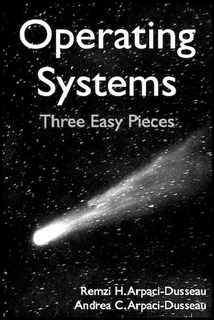
\includegraphics[totalheight=1.5in]{fig/operating-systems.jpeg}\\武汉 $\cdot$ 常州}
\maketitle
% -----------------------------------------------------------------------------------
                         %封面
\include{preface/intro}                          %简介
%\markboth{序}{序} \vspace*{0.0cm}
\thispagestyle{empty}
\vspace*{2.2cm}
\centerline{\zihao{2}\hei{\color{darkblue}{第二版序}}}\vspace{2cm}

吕同富教授编著的《数值计算方法》
………………………………………………


\vspace{2cm}

\hfill XXXXXX\hspace{0.2em}

\hfill 2012年08月于XXXXXX\hspace{0.2em}
                        %序
\markboth{致教育工作者}{致教育工作者} \vspace*{0.0cm}
\thispagestyle{empty}
%\vspace*{2.2cm}
\centerline{\hei{\Large 致教育工作者}}\vspace{2cm}

如果你是希望使用本书的讲师或教授,随时欢迎。可能你已经注意到,本书是免费的,且可以从下面网页中获取:\\
http://www.ostep.org\\
你也可以从lulu.com网站购买纸质版。请在上述网页上查询。

本书的推荐引用格式(截止至目前)如下:\\
~~~~Operating Systems: Three Easy Pieces\\
~~~~Remzi H. Arpaci-Dusseau and Andrea C. Arpaci-Dusseau\\
~~~~Arpaci-Dusseau Books, Inc.\\
~~~~May, 2014 (Version 0.8)\\
~~~~http://www.ostep.org\\

这个课程分成一个学期15周比较好,这样可以覆盖书中的大部分话题,也能达到比较适中的深度。要是把本课程压缩到10周的话,可能需要每个部分都舍弃一些细节。还有一些关于虚拟机监控器的章节,通常压缩到虚拟化的结尾部分或者作为一个aside放在最后。

许多操作系统的书都会将并发性部分放在前面,本书不太一样,将其放在了虚拟化部分之后,这样在此之前可以对CPU和内存的虚拟化有一定理解。从我们15年教授此课程的经验来看,如果学生们没有理解地址空间是什么,进程是什么,或者上下文切换会在任意时间发生,他们都会有个困惑期——不知道并发性问题是如何引起的,为什么要试图解决这个问题。然而,一旦他们理解了虚拟化中的那些概念,当介绍线程和由线程引起的问题时会变得很简单,起码会简单些。

你可能注意到本书没有与之对应的幻灯片。主要原因是我们相信这个过时的教学方法:粉笔和黑板。因此,当我们在讲授这门课程时,我们脑子里带几个主要的思想和一些例子到课堂上,用板书的形式呈现给学生;讲义以及现场编写演示代码也是很有用的。在我们的经验里,使用太多的幻灯片会使得学生心思不在课堂上,因为他们知道反正资料就在这里,可以以后慢慢消化;板书的话会使得课堂像一个现场观看体验,因此会更有互动性、动态性,也会使学生们更好的享受你的课。

如果你想要一份我们上课的笔记的话,可以给我们发邮件。我们已经共享给了全世界很多老师。

最后一个请求:如果你使用网页上的免费章节,请仅仅链接到他们,而不是拷贝到本地。这会帮助我们追踪这些章节的使用情况(过去几年里已经有超过一百万的章节下载量),也可以确保学生们获得的是最新最好的版本。
                   	    %前言
\markboth{致学生}{致~学~生} \vspace*{0.0cm}
\thispagestyle{empty}
%\vspace*{2.2cm}
\centerline{\hei{\Large 致~~学~~生}}\vspace{2cm}

如果你是正在阅读本书的学生,谢谢你!我们很荣幸能够为你提供一些材料帮助你求索关于操作系统的知识。我们俩都很怀念本科时候的一些教科书(如:Hennessy and Patterson [HP90],计算机系统结构的一本经典书),当然也希望本书能够带给你一个美好回忆。

你也许注意到本书是免费的,在网上可以获取到。其主要原因是:教科书一般都比较贵。我们希望,本书能够成为免费书籍新浪潮的第一人,以帮助那些追求自己学业的人。无论他们来自世界的哪个地方或者他们愿意为一本书花多少钱。如若不然,这本免费书也聊胜于无。

可能的话,我们还希望给你们指出书中许多材料的原始出处:那些多年来塑造了操作系统领域的重要的论文和人物。思想不会凭空产生,他们来自于聪明又努力的人(包括许多图灵奖获得者\footnote{图灵奖是计算机科学领域的最高奖;就像诺贝尔奖一样。}),因此我们应该尽可能的去纪念这些思想和人物。在纪念他们时,我们非常希望在写本书时能更好地理解已经发生的革命,而不是仿佛这些思想一直都存在似的[K62]。再者,或许这些参考文献能够促进你自己去更深的挖掘;阅读著名的论文是这个领域最好的学习方法之一。


                     %前言
\markboth{最后的话}{最后的话} \vspace*{0.0cm}
\thispagestyle{empty}
%\vspace*{2.2cm}
\centerline{\hei{\Large 最~后~的~话}}\vspace{2cm}

Yeats【W. B. Yeats,威廉.巴特勒.叶慈】有句名言:”教育不是注满一桶水,而是点燃一把火。”他既是对的但同时也是错的\footnote{如果他确实说了这句话;如许多名人名言一样,这句话的历史也不明}。你必须”注满那桶水”,这些笔记正好在此帮助你的学业;毕竟,当你去Google面试,他们问你一个关于如何使用信号量的刁钻问题,最好还是真的知道信号量是什么,对吧!

但是叶慈的重点明显是:教育真正的关键在于使你能对某样事务产生兴趣,去学习一些自己觉得更重要的东西,而不仅仅是某些课程中为了得高分而需消化的东西。Remzi的父亲曾经说过:”走出课堂学习”。

我们撰写了这些笔记来激发你对操作系统的兴趣,从而去围绕这个话题自己做更多的阅读,去跟你的教授讨论这个领域正在进行的有意思的研究,甚至参与到这个研究中来。这是一个很伟大的领域,充满了精彩美妙思想,它们以深刻而重要的方式塑造了计算机历史。我们知道虽然这把火不能燃烧你们所有人,至少我们希望能够燃烧你们一部分人,甚至几个人。因为一旦这把火被点燃了,那就是你们真正可以做一些伟大事情的时候。教育过程的真正关键是:行动,去研究新的有趣的话题,去学习,去成长,还有最重要的是去寻找能够点燃你的事情。


\vspace{1cm}

\hfill JAndrea and Remzi\hspace{0.2em}

\hfill Married couple \hspace{0.2em}

\hfill Professors of Computer Science at the University of Wisconsin\hspace{0.2em}

\hfill Chief Lighters of Fires, hopefully\footnote{如果这个听起来我们如纵火犯一样在承认一些历史的话,那你可能抓错重点了。也许,如果这听起来俗气的话,那好,因为他就是这么俗气,但你门不得不为此原谅我们。}\hspace{0.2em}


\section*{致谢}
这一节包含了我们对那些帮助撰写本书的人的感谢。现在最重要的事情:你们的名字在这里找到!但是,你一定要帮忙。所以给我们发送一些反馈并帮助我调试本书吧。你可能会出名!或者至少你的名字会出现在本书中。

到目前为止,帮助过本书的人包括: Abhirami Senthilkumaran*, Adam Drescher* (WUSTL), Adam Eggum, Ahmed Fikri*, Ajaykrishna Raghavan, Akiel Khan, Alex Wyler, Anand Mundada, B. Brahmananda Reddy (Minnesota), Bala SubrahmanyamKambala, Benita Bose, BiswajitMazumder (Clemson), Bobby Jack, Bj ¨orn Lindberg, Brennan Payne, Brian Kroth, Cara Lauritzen, Charlotte Kissinger, Chien-Chung Shen (Delaware)*, Christoph Jaeger, Cody Hanson, Dan Soendergaard (U. Aarhus), David Hanle (Grinnell), Deepika Muthukumar, Dorian Arnold (NewMexico), DustinMetzler, Dustin Passofaro, Emily Jacobson, EmmettWitchel (Texas), Ernst Biersack (France), Finn Kuusisto*, Guilherme Baptista, Hamid Reza Ghasemi, Henry Abbey, Hrishikesh Amur, Huanchen Zhang*, Hugo Diaz, Jake Gillberg, James Perry (U.Michigan-Dearborn)*, Jan Reineke (Universit¨at des Saarlandes), Jay Lim, Jerod Weinman (Grinnell), Joel Sommers (Colgate), Jonathan Perry (MIT), Jun He, Karl Wallinger, Kartik Singhal, Kaushik Kannan, Kevin Liu*, Lei Tian (U.Nebraska-Lincoln), Leslie Schultz, LihaoWang, MarthaFerris,Masashi Kishikawa (Sony), Matt Reichoff, Matty Williams, Meng Huang, Mike Griepentrog, Ming Chen (Stonybrook),Mohammed Alali (Delaware),Murugan Kandaswamy, Natasha Eilbert, Nathan Dipiazza, Nathan Sullivan, Neeraj Badlani (N.C. State),
Nelson Gomez, NghiaHuynh (Texas), Patricio Jara, Radford Smith, RiccardoMutschlechner, Ripudaman Singh, Ross Aiken, Ruslan Kiselev, Ryland Herrick, Samer AlKiswany, SandeepUmmadi (Minnesota), Satish Chebrolu (NetApp), Satyanarayana Shanmugam*, Seth Pollen, Sharad Punuganti, Shreevatsa R., Sivaraman Sivaraman*, Srinivasan Thirunarayanan*, Suriyhaprakhas BalaramSankari, SyJinCheah, Thomas Griebel, Tongxin Zheng, Tony Adkins, Torin Rudeen (Princeton), Tuo Wang, Varun Vats, Xiang Peng, Xu Di, Yue Zhuo (Texas A\&M), Yufui Ren, Zef RosnBrick, Zuyu Zhang.

特别感谢Joe Meehean教授(Lynchburg)对每一章的详细注释,Jerod Weinman教授(Grinnell)以及他整个班级不可思议的手册,Chien-Chung Shen教授(Delaware)宝贵细致的阅读和意见,以及Adam Drescher(WUSTL)的仔细阅读和建议。以及所有在资料细化中极大帮助过这些作者的所有人。

同时,也感谢这些年修过537课程的数百名学生。特别的,感谢促使这些笔记第一次成为书面形式的08年秋季班(他们苦于没有任何可阅读的教材——都是有进取心的学生!),并通过赞扬他们使我们能坚持下来(包括那年课程评价里令人捧腹的评价”ZOMG!{典故}你应该写一本全新的教材!")。

当然也亏欠了几个勇敢参与了xv6项目的实验课程的几个人的感谢,其中许多现在已经纳入饿了537主课程中。09年春季班: Justin Cherniak, Patrick Deline, Matt Czech, Tony Gregerson, Michael Griepentrog, Tyler Harter, Ryan Kroiss, Eric Radzikowski, Wesley Reardan, Rajiv Vaidyanathan, and Christopher Waclawik。09年秋季班: Nick Bearson, Aaron  Brown, Alex Bird, David Capel, Keith Gould, Tom Grim, Jeffrey Hugo, Brandon Johnson, John Kjell, Boyan Li, James Loethen,Will McCardell, Ryan Szaroletta, Simon Tso, and Ben Yule.10年春季班: Patrick Blesi, Aidan Dennis-Oehling, Paras Doshi, Jake Friedman, Benjamin Frisch, Evan Hanson, Pikkili Hemanth, Michael Jeung, Alex Langenfeld, Scott Rick, Mike Treffert, Garret Staus, Brennan Wall, Hans Werner, Soo-Young Yang, and Carlos Griffin (almost).

尽管我们的研究生学生没有直接帮助本书的撰写,但是他们教会了我们很多关于这个系统的东西。他们在Wisconsin时,我们经常与他们交流,他们做了所有的实际的工作。并且通过汇报他们做的事情,每周我们也学到了很多新的东西。这个名单包括我们收集到的目前和以前已经发表过论文的学生,星号标记表示那些在我们指导下获得了博士学位的学生: Abhishek Rajimwale, Ao Ma, Brian Forney, Chris Dragga, Deepak Ramamurthi, Florentina Popovici*, Haryadi S. Gunawi*, James Nugent, John Bent*, Lanyue Lu, Lakshmi Bairavasundaram*, Laxman Visampalli, Leo Arulraj, Meenali Rungta,Muthian Sivathanu*, Nathan Burnett*, Nitin Agrawal*, Sriram Subramanian*, Stephen Todd Jones*, Suli Yang, Swaminathan Sundararaman*, Swetha Krishnan, Thanh Do, Thanumalayan S. Pillai, Timothy Denehy*, Tyler Harter, Venkat Venkataramani, Vijay Chidambaram, Vijayan Prabhakaran*, Yiying Zhang*, Yupu Zhang*, Zev
Weiss.

最后还欠Aaron Brown一个感激之情,他多年前第一个带了这门课(09年春),然后有带了xv6实验课(09年秋),最后担任了本课程的研究生助教两年左右(10年秋至12年春)。他的辛勤工作极大的促进了项目的进展(特别是基于xv6的),并因此帮助了Wisconsin的无数的本科生和研究生优化可学习体验。正如Aaron想说的(他一贯的简洁风格):”Thx."

\vspace{1cm}

\hfill Johnnie Xu\hspace{0.2em}

\hfill ****@**** \hspace{0.2em}

\hfill 2015年01月\hspace{0.2em}

%\include{preface/c_abstract}             %中文摘要
%\include{preface/e_abstract}             %英文摘要
%-------------------------------------目录部分------------------------------------------
\setcounter{page}{1}   %重新开始页码
\renewcommand\contentsname{目\qquad 录}
%-------------------下面三行去掉了目录首页页码---------------------
\makeatletter
\let\ps@plain\ps@empty
\makeatother
%-------------------------------------------------------------------------
\tableofcontents                                    %目录
%\addtocontents{toc}{\protect\begin{multicols}{2}}       %目录分两栏开始
\mainmatter    %前言和目录页码结束,正文重新开始设置页码
%-----------------------------------------正文开始------------------------------
%\chapter{本书的一段对话}
\thispagestyle{empty}


\textbf{教授:}欢迎来到这本书!它叫作\textbf{操作系统的三条简洁之道},我在这里会教你们一些你必须了解的操作系统知识。我是「教授」;你们呢?\newline
\textbf{学生:}你好,教授!我是「学生」,你应该猜到了。我在这里准备向您学习。\newline
\textbf{教授:}听起来不错。有什么问题不?\newline
\textbf{学生:}当然,为什么这本书叫作『三条简洁之道』呢?\newline
\textbf{教授:}很简单,你看,这是物理学家理查德·费曼的课程……\newline
\textbf{学生:}哦,是那位写了『别闹了,费曼先生』的那个人吗?好书,这本书是不是也会像那本书一样幽默?\newline
\textbf{教授:}额,不是的。那本书的确很不错,我很高兴你读过那本书。这本书更像他在物理学上的笔记。一些基础被定义为归纳为『六条简洁之道』。他是讨论的物理方面的知识;而我们是讨论以计算机为主题的『三条简洁之道』。差不多,操作系统正好是物理学一半的难度。\newline
\textbf{学生:}那真好,我也喜欢物理。是哪些简洁之道呢?\newline
\textbf{教授:}我们将会学到计算机的三个关键点:『\textbf{虚拟化,并发,持久化}』。在学习这些知识点的时候,我们会了解整个操作系统是如何运作的,包括 CPU 如何决定下一个运行什么程序。如何将内存载入到虚拟内存中。虚拟机监控如何运作,怎样管理硬盘信息,以及一些如何构建部分掉线但仍然可以工作的分布式系统。这是这些东西的主要顺序。\newline
\textbf{学生:}我对您说的这些还没什么概念。\newline
\textbf{教授:}很好,那说明你上对了课了。\newline
\textbf{学生:}我还有另外一个问题:学这些东西最好的方法是什么?\newline
\textbf{教授:}问的好!每个人都需要了解这些,当然,我会这样做:去上课,听教授介绍材料。然后到周末阅读自己的笔记,来帮助你的大脑更深入的理解。一段时间后(提示:在考试之前),再阅读这些笔记来牢固知识。当然,你的教授肯定会布置一些作业和项目,你必须完成;尤其是做项目的时候你为了解决问题而写的代码,是实践笔记中的知识最好的方式。孔子曾经说过……\newline
\textbf{学生:}哦,我知道!『不闻不若闻之,闻之不若见之,见之不若知之,知之不若行之。学至于行之而止矣。』是这句或者类似的吧。\newline
\textbf{教授:}(惊讶)你怎么知道我想说的呢?\newline
\textbf{学生:}因为接下去就像这句啊。而且我非常崇拜孔子,更加崇拜荀子。此句应该是荀子所言。\newline
\textbf{教授:}(震惊)好吧,我想我们要一起好好的努力了。真正的加油。\newline
\textbf{学生:}教授——如果可以的话,我还剩一个问题。这段对话是做什么用的啊?我的意思是,这不应该是一本书吗?为什么不直接介绍实质性的东西呢?\newline
\textbf{教授:}嗯,好问题,好问题!我认为和你自己单独聊这些和思考问题更有用,这段对话就是为了这个。所以你和我要一起工作来完成这个复杂的点子。你准备好了吗?\newline
\textbf{学生:}那我们必须思考?好吧,我准备好了。我的意思是,有一些其他的我能做的吗?貌似我在这本书之外没有太多的出场机会。\newline
\textbf{教授:}不幸的是,我也没有。好了,我们开始工作吧。       %第一章
%\chapter{操作系统介绍}
\thispagestyle{empty}       %第二章
%\include{book/chap3}       %第三章
%\include{book/chap4}       %第四章
%\include{book/chap5}       %第五章
%\include{book/chap6}       %第六章
%\include{book/chap7}       %第七章
%\include{book/chap8}       %第八章
%\include{book/chap9}       %第九章
\chapter{并发性简介}
\thispagestyle{empty}

%\section{引言}
到目前为止,我们已经知道了操作系统基本执行部件的抽象概念的发展。我们已经了解如何『使用』单个物理CPU并将其抽象成多个虚拟CPU,因此多个程序看似同时运行成为了可能【注:在单个单核CPU上,同一时刻实际上只有一个程序在运行】。我们也学习了如何为每个进程构建一个看似很大且私有的虚拟内存;地址空间的抽象概念让每一个程序都好像有了自己的内存,而实际上是操作系统暗地里跨物理内存复用了地址空间(有时是磁盘)。

本节,我们将为单个正在运行的进程引入一个新的概念:线程。不像先前一个程序内只有一个执行点的视角(只从一个PC寄存器取指令和执行指令),一个多线程程序不止一个执行点(多个PC寄存器,可以从每一个PC取指令和执行指令)。从另一个角度来思考这个问题,每一个线程很像一个独立的进程,但是与进程的区别是:进程内的各个线程共享相同的地址空间。所以各个线程可以访问相同的数据。

单个线程的状态与进程的状态的很类似,有一个程序计数器(PC)来跟踪程序从何处取指令。每个线程有自己的用于计算的寄存器集;因此,如果在单个处理器上运行着两个线程,当从一个线程(T1)切换到另一个线程(T2)时,就会发生一次上下文切换。线程的上下文切换跟进程的上下文切换很类似,因为需要保存T1的寄存器状态,并在T2运行之前加载T2的寄存器状态。对于进程来说,我们将状态保存到进程控制块(process control block,PCB);对于线程来说,我们需要一个或多个线程控制块(thread control blocks,TCBs)来存储单个进程中的多个线程的状态。尽管如此,线程间的上下文切换比起进程来,有一个重要区别:地址空间依旧保持不变(没有必要切换正在使用的页表)。

线程与进程之间的另一个重要的区别是栈(stack)。在经典进程(现在可以称之为单线程进程,single-threaded process)地址空间的简单模型中,有一个单独的栈,通常位于地址空间的的底端(见下左图)。

\begin{figure}[h]
\centering
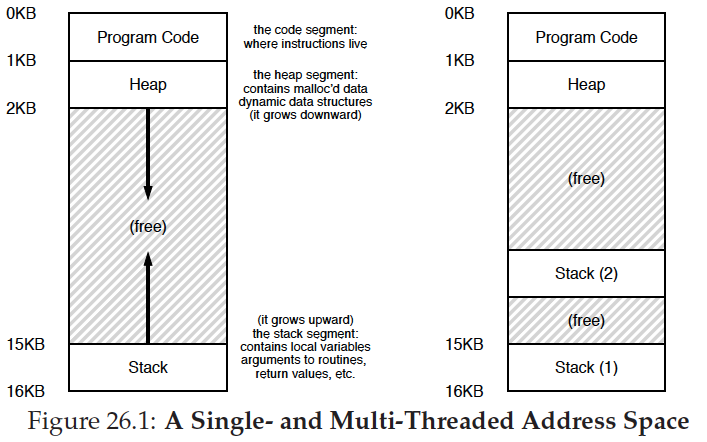
\includegraphics[width=0.75\textwidth]{fig/figure-26-1.png}
\caption{图26.1:单线程和多线程的地址空间} \label{fig:figure-26-1}
\end{figure}

然而,在多线程进程中,每个线程独立运行,当然会调用各种各样的routines来完成它正在做的任何工作。跟地址空间中只有一个栈不同,多线程进程中每个线程都有一个栈。假设一个多线程进程内有两个线程,其相应的地址空间与经典进程不一样(见上右图)。

在Figure26.1中,可以看到两个栈分布在进程的"整个"地址空间中。因此,任何在栈中分配的变量、参数、返回值以及其他存放在栈中的数据将会存储在那个有时称作线程局部空间的地方,即相应线程的栈。

也许你也注意到了新的布局破坏了原来"美观"的地址空间布局。之前,堆栈可以各自独立增长而不出问题,除非超出了地址空间的范围。而现在的地址空间布局就不再有先前的"nice situation"。幸运的是,这样的空间布局通常是可行的,因为栈一般不需要特别大(程序大量使用递归时除外)。

\section{例子:线程创建}
假设我们想运行一个创建两个线程的程序,每个线程各自执行相互独立的任务,打印「A」或「B」。代码如Figure 26.2所示。

主程序创建两个线程,每个都执行函数mythread(),但是传递不同的参数(字符串『A』或『B』)。一旦创建了线程,它可能会立即运行(取决于调度器的whims);也可能会进入『就绪』态而非『运行』态,因此不立即执行。创建两个线程之后(T1和T2),主线程调用pthread\_join()等待对应的线程结束。
\begin{figure}[t]
\begin{lstlisting}
#include <stdio.h>
#include <assert.h>
#include <pthread.h>

void *mythread(void *arg) {
    printf("%s\n", (char *) arg);
    return NULL;
}

int
main(int argc, char *argv[]) {
    pthread_t p1, p2;
    int rc;
    printf("main: begin\n");
    rc = pthread_create(&p1, NULL, mythread, "A"); assert(rc == 0);
    rc = pthread_create(&p2, NULL, mythread, "B"); assert(rc == 0);
    // join waits for the threads to finish
    rc = pthread_join(p1, NULL); assert(rc == 0);
    rc = pthread_join(p2, NULL); assert(rc == 0);
    printf("main: end\n");
    return 0;
}
\end{lstlisting}
\caption{简单的线程创建代码}
\end{figure}

我们来看一下这个小程序可能的执行顺序,在执行示意图中(表 26.1),时间从上向下依次增长,每一栏显示了什么时候运行不同的线程(主线程、线程T1、或线程T2)。

然而,注意这个顺序并不是唯一的执行顺序。实际上,对于一个给定的指令序列,它有不少的可能执行顺序,这取决于在特定的时刻调度器决定哪个线程能得到执行。比如,一旦创建了一个线程,它可能立即执行,如表26.2所示的执行顺序。

我们也可以看到『B』在『A』之前打印出来,这就是说调度器决定先执行线程T2,即使线程T1更早创建;没有任何理由取假设先创建的线程就先运行。表26.3显示了这个执行顺序,线程T2*******with Thread 2 getting to strut its stuff before Thread 1.

As you might be able to see, one way to think about thread creation is that it is a bit like making a function call; however, instead of first executing the function and then returning to the caller, the system instead creates a new thread of execution for the routine that is being called, and it runs independently of the caller, perhaps before returning from the create, but perhaps much later. 

As you also might be able to tell from this example, threads make life complicated: it is already hard to tell what will run when! Computers are hard enough to understand without concurrency. Unfortunately, with concurrency, it gets worse. Much worse.

\begin{table}[p]
\centering
{\scriptsize
\begin{tabular}{p{5cm} l l}
\textbf{main}&\textbf{Thread 1}&\textbf{Thread 2}\\ \midrule[1.1pt]
starts running &  & \\
prints "main:begin" &  & \\
creates Thread 1&  &  \\
creates Thread 2&  &  \\
waits for T1&  &  \\
  & runs &  \\
  & prints "A" &  \\
  & returns &  \\
waits for T2 &  &  \\
  &  & runs \\
  &  & prints "B" \\
  &  & returns \\
prints "main:end" &  &  \\
\end{tabular}}
\caption{\footnotesize 线程执行轨迹(1)}\color{black}\label{tab26-1}

\vspace{0.5cm}
{\scriptsize
\begin{tabular}{p{5cm} l l}
\textbf{main}&\textbf{Thread 1}&\textbf{Thread 2}\\ \midrule[1.1pt]
starts running &  & \\
prints "main:begin" &  & \\
creates Thread 1&  &  \\
  & runs &  \\
  & prints "A" &  \\
  & returns &  \\
creates Thread 2&  &  \\
  &  & runs \\
  &  & prints "B" \\
  &  & returns \\
waits for T1&  &  \\
\textsl{~~~~returns immediately; T1 is done} &  & \\
waits for T2 &  &  \\
\textsl{~~~~returns immediately; T2 is done} &  & \\
prints "main:end" &  &  \\
\end{tabular}}
\caption{{\footnotesize 线程执行轨迹(2)}}\color{black}\label{tab26-1}

\vspace{0.5cm}
{\scriptsize
\begin{tabular}{p{5cm} l l}
\textbf{main}&\textbf{Thread 1}&\textbf{Thread 2}\\ \midrule[1.1pt]
starts running &  & \\
prints "main:begin" &  & \\
creates Thread 1&  &  \\
creates Thread 2&  &  \\
  & runs &  \\
  & prints "A" &  \\
  & returns &  \\
waits for T1 &  &  \\
  &  & runs \\
  &  & prints "B" \\
  &  & returns \\
waits for T2 &  &  \\
\textsl{~~~~returns immediately; T2 is done} &  & \\
prints "main:end" &  &  \\
\end{tabular}}
\caption{\footnotesize 线程执行轨迹(3)}\color{black}\label{tab26-1}
\end{table}

\clearpage


\begin{lstlisting}
#include <stdio.h>
#include <pthread.h>
#include "mythreads.h"

static volatile int counter = 0;

/* Simply adds 1 to counter repeatedly, in a loop. No, this is not how 
 * you would add 10,000,000 to a counter, but it shows the problem nicely. */

void *mythread(void *arg) {
    printf("%s: begin\n", (char *) arg);
    int i;
    for (i = 0; i < 1e7; i++) {
        counter = counter + 1;
    }
    printf("%s: done\n", (char *) arg);
    return NULL;
}

/* Just launches two threads (pthread_create) and then waits for them (pthread_join) */

int main(int argc, char *argv[]) {
    pthread_t p1, p2;
    printf("main: begin (counter = %d)\n", counter);
    Pthread_create(&p1, NULL, mythread, "A");
    Pthread_create(&p2, NULL, mythread, "B");

    // join waits for the threads to finish
    Pthread_join(p1, NULL);
    Pthread_join(p2, NULL);
    printf("main: done with both (counter = %d)\n", counter);
    return 0;
}
\end{lstlisting}

%\begin{figure}[h]
%\caption{共享数据}
%\end{figure}

\section{为何更糟糕:共享数据}
上一节简单的线程示例可以有效的解释线程是如何被创建,以及它们是如何按照不同的顺序运行,这个执行顺序决定于调度器决定如何运行它们。这个示例并没有展示线程间在访问共享数据时是如何交互的。

让我们设想一个简单的例子:有两个线程想要更新一个全局共享变量。我们将要研究的代码见Figure 26.3。

有几个关于这段代码的注释。第一,如Stevens的建议【SR05】,我们封装了线程的create和join例程与其失败退出判断【***】,对于一个简单如此的程序,我们至少要关注发生的错误(如果发生的话),但是不做任何很【smart】的事儿(如:仅仅退出)。因,Pthread\_create()简单的调用pthread\_create()并确定返回值为0;如果不是,Pthread\_create()仅仅打印一个消息并退出。

第二,这个例子为工作线程仅用一个函数而不是两个独立的函数(即两个线程执行同一个函数,译者注),向线程传递一个参数(这里是字符串)让每一个线程在其消息之前打印不同的字母。

最后也是最重要的,我们可以看每个工作线程试图做的事:共享变量counter加1,这个操作在循环中执行一千万次。因此,理想的最终结果是:20,000,000。

现在编译执行这个程序,看一下它的结果。有时候,everything works how we might expect:
\begin{verbatim}
prompt> gcc -o main main.c -Wall -pthread
prompt> ./main
main: begin (counter = 0)
A: begin
B: begin
A: done
B: done
main: done with both (counter = 20000000)
\end{verbatim}

不幸的是,当我们运行这段代码时,即使是在一个处理器上,我们也得不到那个预期的结果。有时,结果如下:
\begin{verbatim}
prompt> ./main
main: begin (counter = 0)
A: begin
B: begin
A: done
B: done
main: done with both (counter = 19345221)
\end{verbatim}

我们再试一次,看看是不是我们疯狂了。毕竟,如你所接受的教育,计算机并不认为会产生确定性结果。也许你的处理器欺骗了你?(等我喘口气)
\begin{verbatim}
prompt> ./main
main: begin (counter = 0)
A: begin
B: begin
A: done
B: done
main: done with both (counter = 19221041)
\end{verbatim}

不仅每一个都是错误的结果,而且每个结果还不一样!大大的疑问:为什么会发生这样的事儿呢?

\begin{tcolorbox}[colframe=grey,colback= grey,arc=0pt,left=6pt,right=6pt,top=6pt,bottom=6pt,boxsep=0pt]
\begin{center}技巧:了解并使用你的工具
\end{center}

你总是需要学习心得工具来帮助你编写、调试和理解计算机系统。这里我们使用一个小巧的工具:反汇编器(disassembler)。当你对一个可执行文件执行反汇编时,它会显示这个可执行文件是有哪些会变代码组成的。例如,如果你希望理解例子中更新counter的底层代码,运行objdump(Linux)来它的汇编代码:
\begin{verbatim}
prompt> objdump -d main
\end{verbatim}
\end{tcolorbox}

\section{核心问题:失控的调度}
为了理解为何会发生这样的事儿,我们需要理解编译器为更新counter而生成的指令序列。在这个例子里,我们希望简简单单的将counter加1。因此,做这一操作的指令序列也许应该如下(x86):
\begin{verbatim}
mov 0x8049a1c, %eax
add $0x1, %eax
mov %eax, 0x8049a1c
\end{verbatim}

这个例子假设变量counter分配的地址是0x8049a1c。在这个三指令的序列里,x86的mov指令首先取得该地址的内存值并将其放入寄存器eax中,然后,执行add操作,eax寄存器的值加1,最后,eax的值写回原先的内存地址。

我们设想一下两个线程中的一个(线程T1)进入这段代码,它对counter执行了加1操作。它首先加载counter的值(假设其初值是50)进入寄存器eax,因此对线程T1来说寄存器eax的值为50。然后它对寄存器执行加1操作,此时eax的值是51。现在,发生了件不幸的事儿:定时器中断到达;因此,操作系统保存当前运行线程的状态(PC,eax等寄存器)至线程的TCB。

现在发生了更糟糕的事儿:线程T2被调度执行,它进入同一段代码。它也执行第一条指令,获取counter的值并写入它的eax寄存器(注:每个线程在运行时都有自己私有的寄存器;这些寄存器是通过上下文切换代码保存、加载虚拟化出来)。counter的值此时仍然是50,因此线程T2的eax值为50。假设线程T2继续执行接下来的两条指令,eax加1(eax=51),然后保存eax的内容至counter(内存地址0x8049a1c)。因此,全局变量counter此时的值是51。

最后,又一次发生上下文切换,并且线程T1得到了执行。记得刚才仅仅执行过了mov和add指令,那么此时应当执行最后一条mov指令。刚才eax的值是51,因此,最后执行mov指令并将值写入内存;counter的又一次被写为51。

简单的说,事儿是这样的:counter加1的代码执行了两次,但是初值为50的counter现在只有51。但是这个程序『正确的』结果应当是变量counter值为52。

我们来看一下详细的执行路径以便更好的理解这个问题。对于这个例子,假设上述的代码加载到内存地址100处,如下图所示的指令序列(注意那些曾经优秀的精简指令集:x86有变长指令;这里的mov指令占5字节的内存,add指令仅占3字节):
\begin{verbatim}
100 mov 0x8049a1c, %eax
105 add $0x1, %eax
108 mov %eax, 0x8049a1c
\end{verbatim}
基于这些假设,上述发生的事儿如表26.4所示。假设counter起始值是50,然后跟踪这个例子确保你可以理解正在发生什么。
\begin{table}[h]
{\footnotesize
\begin{tabular}{p{3cm} p{3cm} p{3cm} c c c}
 & & & \multicolumn{3}{c|}{after instruction} \\
\textbf{OS}&\textbf{Thread 1}&\textbf{Thread 2} & \textbf{PC}  & \textbf{\%eax} & \textbf{counter}\\
\midrule[1.1pt]
 & before critical section &  & 100 & 0 & 50 \\
 & mov 0x8049a1c, \%eax  &  & 105 & 50 & 50\\
 & add \$0x1, \%eax &  & 108 & 51 & 50 \\
 \textbf{interrupt} & & & & & \\
 ~~~~\textsl{save T1's state} & & & & & \\
 ~~~~\textsl{restore T2's state} & & & 100 & 0 & 50 \\
  & & mov 0x8049a1c, \%eax & 105 & 50 & 50 \\
  & & add \$0x1, \%eax & 108 & 51 & 50 \\
  & & mov \%eax, 0x8049a1c & 113 & 51 & 51 \\
\textbf{interrupt} & & & & & \\
 ~~~~\textsl{save T2's state} & & & & & \\
 ~~~~\textsl{restore T1's state} & & & 108 & 51 & 50 \\
  & mov \%eax, 0x8049a1c & & 113 & 51 & 51 \\
\end{tabular}}
\caption{问题:up close and personal}\color{black}\label{tab26-1}
\end{table}

上面已经示范的问题称作:竞争条件,其结果取决于这段代码的执行时机。有时候运气不好(例如:在执行的时候发生不合时宜的上下文切换),就会得到错误的结果。实际上,我们很可能每次都得到不同的值;因此,而不是确定性计算(曾经来源于计算机??),我们称之为不确定性,不知道输出的会是什么,且这些输出在交叉运行之间很可能会不同。

因为多线程执行这段代码会引起竞争条件,我们称这段代码为:临界区。一个临界区是一段访问共享变量(更一般的;共享资源)且不可被多于一个线程并发执行的代码段。

对于这段代码,我们需要的是称之为互斥量的东西。这个性质保证了如果有一个线程正在执行临界区代码,其他的线程都会被阻止进入临界区。

顺便提一下,实际上所有这些概念都是由Edsger Dijkstra创造出来的。他是这个领域的开拓者,并凭借这个工作和其他成果获得了图灵奖;详见他1968年的论文『Cooperating Sequential Processes』[D68]中对此问题惊人清晰的描述。我们还会在本章中多次看见Dijkstra。

\section{原子性的愿望}
解决这个问题的一个办
法是更强大的指令,这些指令可以在单步之内做任何我们需要做的,因此避免了发生不合时宜的中断的可能性。例如,假如我们有一个像下面所示一样的超级指令,会怎样呢?
\begin{verbatim}
memory-add 0x8049a1c, $0x1
\end{verbatim}

假设这条指令将一个值加到该内存地址,并硬件保证它是原子执行的;当这条指令执行后,它将按照预想的那样执行更新操作。它不会在指令执行中被中断,因为正是我们从硬件那儿得到的保证:当中断发生时,这条指令要么没有执行,要么已经执行结束;没有中间状态。硬件可以如此的美好,不是么?

在此文中,原子性意味着『作为一个单位』,有时称之为『全或无』。我们想原子地执行这三条指令序列:
\begin{verbatim}
mov 0x8049a1c, %eax
add $0x1, %eax
mov %eax, 0x8049a1c
\end{verbatim}

如之前所说的,如果有一条单独指令能够完成这个操作,那么只需要发出指令即可完成。但是通常情况下,没有这样的指令。设想我们已经构建了一个并发的B树,此时想要更新它;难道要硬件支持『B树的原子更新』指令么?恐怕不可能,至少在合理的指令集中是如此。

因此,相反的,由硬件提供少量有效的指令,我们可以借助这些指令构建一系列通用的同步原语。通过这些硬件同步原语与操作系统的支持,我们可以构造出以同步可控方式访问临界区的多线程代码,因此可以可靠的生成正确的结果,尽管存在并发执行的挑战。相当的棒,是不?

这是本节将要研究的问题。这是一个奇妙也很难的问题,应该会让你(有点)头疼。如果没有头疼,那就是你没懂!继续研究直到你头疼为止,那时候你就知道自己已经走向了正确的方向。到了那个时候,休息一会儿,我们可不想让你头疼的厉害。
\begin{tcolorbox}[colframe=grey,colback= grey,arc=0pt,left=6pt,right=6pt,top=6pt,bottom=6pt,boxsep=0pt]
\begin{center}症结所在:如何为同步提供支持\end{center}

为了构建有效的同步原语,我恩需要硬件提供什么支持呢?又需要操作系统提供什么支持呢?我们怎么才能正确高效的构建这些原语呢?程序又如何使用他们以得到期望的结果呢?
\end{tcolorbox}

\begin{tcolorbox}[colframe=grey,colback= grey,arc=0pt,left=6pt,right=6pt,top=6pt,bottom=6pt,boxsep=0pt]
\begin{center}
关键并发术语\\
临界区,竞争条件,不确定性,互斥
\end{center}
这四个术语对于并发代码太核心了,以至于我认为非常值得把它们提出来说一下。详见Dijkstra早期的工作[D65,D68]。
\begin{itemize}
\item 临界区,临界区是一段访问共享资源的代码段,共享资源一般是一个变量或数据结构
\item 竞争条件,竞争条件发生在正在执行的多个线程几乎同时进入临界区;多个线程都试图更新共享数据结构,同时导致产生奇怪(可能非预期)的结果。
\item 不确定性,一段不确定的程序有一个或多个竞争条件组成,一次一次执行的输出变化不一,视不同线程何时运行而定。因此结果是不确定的,通常我们指望着计算机系统。
\item 互斥,为了避免这个这些问题,线程需要使用某种互斥原语;以此保证只有一个线程已经进入临界区,从而避免竞争得到确定性的结果。
\end{itemize}
\end{tcolorbox}

\section{另一个问题:等待其他线程}
本章所设定的并发问题,线程间貌似只有一种交互形式,即访问共享变量以及临界区原子性的支持。事实证明,还会产生另一种常见的交互,即一个线程必须等待其他线程完成某些操作方能继续执行。例如,当一个进程执行磁盘I/O时而休眠时,这种交互就会产生;当磁盘I/O完成时,进程需要从休眠中唤醒以便继续执行。
因此,在接下来的章节中,我们不仅仅会研究如何构建同步原语为原子性提供支持,还会研究相应的机制来为多线程程序中常见的休眠唤醒交互方式提供支持。
要是现在这东西没有意义,那好!当你读到条件变量那章时就会觉得有意义了。如果那时觉得不太行,那你应该一遍再一遍的读那章直到觉得有意义。

\section{小结:为什么在OS级}
在wrapping up之前,你可能有一个疑问:为什么我们要在OS这一层研究这些?答案就一个词——历史;操作系统是第一个并发程序,许多技术都被创造用于OS中。后来,在多线程进程中,应用程序编写者也不得不考虑这些事儿。

例如,设想这样的场景,有两个正在运行的进程。假如它们都调用write()来写一个文件,都想将数据附加到文件中(例如:添加数据到文件末尾,从而增加它的长度)。这样的话,两者都需要分配一个新的块,记录块的位置到文件的inode中,并改变文件大小以示一个更大的大小(我们将会在本书第三部分学到更多关于文件的内容)。因为中断可能随时都会发生,更新这些共享数据结构的代码就是临界区,因此,从最开始的中断介绍可知,操作系统设计者不得不担心操作系统怎么更新这些内部结构。一个不合时宜的中断引起了上述的所有问题。不奇怪,页表,进程列表,文件系统结构等。实际上,所有内核数据结构都需要通过合适的同步原语来谨慎访问,以便正确工作。

\begin{tcolorbox}[colframe=grey,colback= grey,arc=0pt,left=6pt,right=6pt,top=6pt,bottom=6pt,boxsep=0pt]
\begin{center}技巧:使用原子操作\end{center}
原子操作是构建计算机系统最强大的底层技术之一,从计算机体系结构到并发代码(本节正在研究的)、文件系统(后面将会研究的)、数据库管理系统,甚至分布式系统[L+93]。
使得一系列行为原子化背后的思想可以简单的缩成一个短语——全或无。你希望一起执行的行为要么全都发生了,要么全都没有发生,而没有中间状态。有时,将许多行为组织成一个原子行为称作:事务,这个思想在数据库和事务处理领域已经发展很成熟[GR92]。
在探索并发性的主题中,我们会使用同步原语把短指令序列转化成原子执行块。但是如我们将会见到的,原子性的思想远不止这些。例如,文件系统使用诸如日志或copy-on-write等技术来原子地转移它们的磁盘状态,使得在面对系统故障时能严格正确地执行。If that doesn’t make sense, don’t worry—it will, in some future chapter。
\end{tcolorbox}



\chapter{插曲:线程API}
\thispagestyle{empty}

本章简要讲解线程API的主要内容。每个部分将会按照介绍如何使用这些API的顺序,在后续章节进行详细解释。更多的细节可以在许多书和在线资源里找到[B97,B+96,K+96]。需要注意,由于有很多的例子,接下来锁和条件变量概念的章节讲起来会很慢;因此,本章用作一个引用会更好些。

\begin{tcolorbox}[colframe=grey,colback= grey,arc=0pt,left=6pt,right=6pt,top=6pt,bottom=6pt,boxsep=0pt]
\begin{center}关键:如何创建并控制线程
\end{center}
操作系统应该为线程创建和控制提供什么接口?应该如何设计这些接口,使之跟一般程序接口一样使用自如?
\end{tcolorbox}

\section{线程创建}
编写多线程程序,首先要做的就是创建新线程;因此,需要存在某种线程创建接口。在POSIX中,很简单:
\begin{verbatim}
#include <pthread.h>
int  pthread_create( pthread_t * thread,  const pthread_attr_t * attr,
                     void * (*start_routine)(void*),  void * arg);
\end{verbatim}
这个声明貌似有点小复杂(特别是当你没有用过C语言的函数指针),其实这并不糟糕。这里有四个参数:thread,attr,start\_routine,arg。第一个参数thread是一个指向pthread\_t结构体的指针;我们将会用这个结构体与起对应的线程进行交互,因此我们需要将它传给pthread\_create()函数初始化。

第二个参数attr,用来指定一些这个线程可能需要的一些属性。比如设置栈大小,或者这个线程的调度优先级的信息等。可以单独调用pthread\_attr\_init()函数来初始化一个属性;欲知详情,请查阅对应手册。然而,许多情况下,默认属性就可以了,这样的话,给该参数传递一个NULL即可。

第三个参数是最复杂的,实际上它只是想知道:这个线程从哪个函数开始运行?在C语言中,称之为函数指针。这个函数指针告诉我们一下信息:函数名(start\_routine),传递给该函数一个void *类型的参数(如start\_routine括号之后表示的),以及该函数一个类型为void *的返回值(例如:空指针)。

如果这个函数指针想要的不是空指针,而是一个整型参数,其声明如下:
\begin{verbatim}
int pthread_create(..., // 前两个参数一样
                    void * (*start_routine)(int), int arg);
\end{verbatim}
如果函数指针希望传一个空指针参数,但是要返回一个整型值,则其声明如下:
\begin{verbatim}
int pthread_create(..., // 前两个参数一样
                    int (*start_routine)(void *), void * arg);
\end{verbatim}

最后,第四个参数arg实际上就是传递个函数指针的参数。你可能会有疑问:为什么需要这些空指针呢?其实答案很简单:start\_routine函数有了一个空指针作为参数,就可以传递任意类型的参数给它了;有一个空指针的返回值就允许线程返回任意类型的结果。
\begin{figure}[h]
\begin{lstlisting}
#include <pthread.h>

typedef struct __myarg_t {
	int a;
	int b;
}myarg_t;

void *mythread(void *arg) {
	myarg_t *m = (myarg_t *) arg;
	printf("%d %d\n", m->a, m->b);
	return NULL; 
}

int main(int argc, char *argv[]) {
	pthread_t p;
	int rc;
	myarg_t args;
	args.a = 10;
	args.b = 20;
	rc = pthread_create(&p, NULL, mythread, &args);
	...
}
\end{lstlisting}
\caption{创建线程}
\end{figure}

我们来看图27.1的例子。仅创建了一个传递了两个参数的线程,这两个参数组成自己定义的类型(myarg\_t)。一旦创建后,这个线程就可以简单地将它的参数转化成想要的类型,并可按预期得到这些参数。

一旦创建了线程,就会存在一个新的存活的执行实体,与它自己的调用栈一起完成,跟程序中所有存在的线程一样运行在相同的地址空间。快乐之旅由此开始!

\begin{lstlisting}
#include <stdio.h>
#include <pthread.h>
#include <assert.h>
#include <stdlib.h>

typedef struct __myarg_t {
	int a;
	int b;
} myarg_t;
typedef struct __myret_t {
	int x;
	int y;
} myret_t;

void *mythread(void *arg) {
	myarg_t *m = (myarg_t *) arg;
	printf("%d %d\n", m->a, m->b);
	myret_t *r = Malloc(sizeof(myret_t));
	r->x = 1;
	r->y = 2;
	return (void *) r;
}

int main(int argc, char *argv[]) {
	int rc;
	pthread_t p;
	myret_t *m;

	myarg_t args;
	args.a = 10;
	args.b = 20;
	Pthread_create(&p, NULL, mythread, &args);
	Pthread_join(p, (void **) &m);
	printf("returned %d %d\n", m->x, m->y);
	return 0;
}
\end{lstlisting}
\begin{figure}[h]
\setlength{\abovecaptionskip}{1pt}
\caption{等待线程完成}
\setlength{\belowcaptionskip}{1pt}
\end{figure}

\section{线程完成(completion)}
之前的例子展示了如何创建一个线程。然而,如果想要等待一个线程的完成会发生什么呢?你需要做一些特别的事儿来等待线程完成;特别的,你需要调用的pthread\_join()函数。
\begin{verbatim}
int pthread_join(pthread_t thread, void **value_ptr);
\end{verbatim}
这个函数只有两个参数,第一个参数是pthread\_t类型,用来指定要等待哪个线程。实际上就是在创建线程时传递给线程库的那个值;如果持有这个值,那么现在就可以用来等待那个线程的运行终止。

第二个参数是一个指向你想要取回的返回值的指针。因为这个函数可以返回任意值,故其定义成了一个空指针;由于pthread\_join会改变传给它的参数,故应该传递该值的指针,而不是值本身。

我们来看另外一个例子(图27.2)。在这段代码里,还是创建了一个线程,并通过myarg\_t结构体传递了一对参数。返回值用到了myret\_t类型。一旦这个线程结束运行,正等在pthread\_join()的主线程就会返回,并且可以访问从线程返回的值,即myret\_t里的内容。



这个例子有几个注意点。第一,大多数时候我们不需要做所有这些痛苦的 packing and unpacking of arguments的事儿。例如,如果我们仅需创建一个无参的线程,传递一个NULL作为参数即可。类似的,如果我们不关心返回值的话,可以给pthread\_join()传一个NULL。
第二,如果我们仅传一个值的话(如int),就不需要package它作为一个参数。图27.3就是一个例子。这种情况下,由于我们不需要将参数和返回值package成结构体,就简单了很多。

\begin{figure}[h]
\begin{lstlisting}
void *mythread(void *arg) {
	int m = (int) arg;
	printf("%d\n", m);
	return (void *) (arg + 1);
}

int main(int argc, char *argv[]) {
	pthread_t p;
	int rc, m;
	Pthread_create(&p, NULL, mythread, (void *) 100);
	Pthread_join(p, (void **) &m);
	printf("returned %d\n", m);
	return 0;
}
\end{lstlisting}
%\setlength{\abovecaptionskip}{2pt}
\caption{等待线程完成}
\end{figure}

第三,需要非常注意返回值是如何从线程返回的。尤其,不要返回一个指向了线程调用栈中分配的值的指针。如果这么做了,你觉得会发生什么呢?(考虑一下)这里是一段问题代码的例子,改自图27.2中的例子。

\begin{verbatim}
void *mythread(void *arg) {
    myarg_t *m = (myarg_t *) arg;
    printf("%d %d\n", m->a, m->b);
    myret_t r; // 分配在栈中: BAD!
    r.x = 1;
    r.y = 2;
    return (void *) &r;
}
\end{verbatim}

在这种情况下,变量r是在mythread的栈中分配的。然而,当线程返回时,这个值会自动释放(这就是为什么栈使用起来这么简单)。因此,传回去的指针就是一个未分配的变量,可能会导致各种错误结果。当然,当你输出你觉得你返回了的值时,你很可能(不一定)会感到奇怪。可以自己试试看!【2. 幸运的是当你这样的代码时,编译器gcc可能会抱怨的,这也是一个注意编译器警告的原因】

最后,你可能注意到使用pthread\_create()创建线程之后,紧接着就调用了pthread\_join(),这种创建线程的方式很奇怪。实际上,有一种更容易的方式来完成这样的任务,叫做过程调用。通常我们会创建不止一个线程并等待它完成,否则完全没有使用多线程的意义。

我们应该注意到并不是所有的多线程代码都使用join函数。例如,一个多线程web服务器可能创建多个工作线程(worker),然后使用主线程accept请求并将之传给工作线程(worker)。因此,这样长生存期的程序也许就不需要join。然而,一个创建多个线程去并行执行特定任务并行程序很可能会用join来确保所有的工作都完成,才退出或进入下一阶段工作。

\section{锁}
除了线程创建(creation)和合并(join),也许,POSIX线程库提供的最有用的一些列函数是通过锁(locks)来为临界区提供互斥量的函数。这对最基础的函数由下列两个函数提供:
\begin{verbatim}
int pthread_mutex_lock(pthread_mutex_t *mutex);
int pthread_mutex_unlock(pthread_mutex_t *mutex);
\end{verbatim}

这两个函数应该很容易理解和使用。当你实现的一段代码是临界区时,需要用锁来保护以使按照预期执行。你大概可以想象一下,代码应该如下:
\begin{verbatim}
pthread_mutex_t lock;
pthread_mutex_lock(&lock);
x = x + 1; // or whatever your critical section is
pthread_mutex_unlock(&lock);
\end{verbatim}

这段代码的意思是这样的:如果在调用pthread\_mutex\_lock()时没有其他的线程持有这个锁,这个线程就取获取这个锁,并进入临界区。如果其他线程已经持有这个锁,则这个试图获取锁的线程会阻塞直到获取到锁(意味着那个持有锁的线程已经调用unlock释放了这个锁)。当然,有可能在一个给定的时间会有很多线程卡在线程获取函数;只有那个获取到锁的调用unlock。【*****】

可惜,这段代码在两个地方有问题。第一个问题是:未有合适的初始化。所有的锁都必须被正确地初始化,以保证它们都有正确的初始值,以及在调用lock和unlock时能够正常工作。

在POSIX线程中,有两种初始化锁的方式。一种是用 PTHREAD\_MUTEX\_INITIALIZER来初始化,如下:
\begin{verbatim}
pthread_mutex_t lock = PTHREAD_MUTEX_INITIALIZER;
\end{verbatim}

这种方式将锁设置为默认值并设为可用。另一种动态方式是调用 pthread\_mutex\_init(),如下:
\begin{verbatim}
int rc = pthread_mutex_init(&lock, NULL);
assert(rc == 0); // always check success!
\end{verbatim}

第一个参数是锁的地址,而第二个参数是一个可选的属性集。关于该属性集可以自己查阅;简单地传递NULL则是使用默认方式。上述的两种方式都可以,但我们通常使用动态的方法(后者)。注意,当锁使用结束时,相应的要调用 pthread\_mutex\_destroy()。可参见相应的手册获取这部分的所有细节。

第二个问题是没有检测lock和unlock调用的错误码。就像你在UNIX系统中调用几乎所有的库函数一样,这些函数也可能失败!如果你的代码没有正确的检测错误码,那么错误就会默默的发生,这种情况下就有可能多个线程都进入了临界区。最起码,要用断言将其封装(如图27.4);更多的成熟(non-toy)的程序,在出错时不能简单的退出,当lock和unlock失败时,应当检测错误并采取一些适当措施。

\begin{figure}[h]
\begin{verbatim}
// Use this to keep your code clean but check for failures
// Only use if exiting program is OK upon failure
void Pthread_mutex_lock(pthread_mutex_t *mutex) {
    int rc = pthread_mutex_lock(mutex);
    assert(rc == 0);
}
\end{verbatim}
\setlength{\abovecaptionskip}{2pt}
\caption{简单封装}
\end{figure}

lock和unlock函数并不是pthreads仅有的锁相关函数。特别的,还有两个函数可能感兴趣函数:
\begin{verbatim}
int pthread_mutex_trylock(pthread_mutex_t *mutex);
int pthread_mutex_timedlock(pthread_mutex_t *mutex,
                            struct timespec *abs_timeout);
\end{verbatim}
这两个函数在获取锁时使用。trylock函数会在锁已经被持有时返回失败;timedlock函数会在得到了锁或者超时之后返回,无论那个先发生。因此,timedlock函数在超时值为0时退化成trylock函数。一般讲,要避免使用这两个函数;然而,有少部分时候为了避免阻塞在获取锁上,这两函数还是很有用的,正如下一章我们将讲到的(如:当我们研究死锁时)。

\section{条件变量}
线程库的另一个主要组件就是条件变量,当然POSIX线程也是这样。当某种信号必须在信号间发生时,条件变量是很有用的,如一个线程需要等待其他线程完成某事才能继续执行。程序希望以这种方式交互时,会常用两个函数:
\begin{verbatim}
int pthread_cond_wait(pthread_cond_t *cond, pthread_mutex_t *mutex);
int pthread_cond_signal(pthread_cond_t *cond);
\end{verbatim}

要使用条件变量,另外还需要有一个与之关联的锁。当调用这两个函数时,都要先持有对应的锁。

第一个函数,pthread\_cond\_wait(),会使调用线程休眠,等待其他线程唤醒它,通常是这个休眠的线程关心的某些事发生了改变。例如,典型的使用如下:
\begin{verbatim}
pthread_mutex_t lock = PTHREAD_MUTEX_INITIALIZER;
pthread_cond_t init = PTHREAD_COND_INITIALIZER;
Pthread_mutex_lock(&lock);
while (initialized == 0)
     Pthread_cond_wait(&init, &lock);
Pthread_mutex_unlock(&lock);
\end{verbatim}

这段代码,在初始化了相关的锁和条件变量之后,线程检测变量initialized是否已经被设置为其他值而非0。如果没有,线程就简单的调用wait函数休眠,直到其他线程唤醒它。

其他线程中唤醒这个线程的代码如下:
\begin{verbatim}
Pthread_mutex_lock(&lock);
initialized = 1;
Pthread_cond_signal(&init);
Pthread_mutex_unlock(&lock);
\end{verbatim}

这段代码的顺序有几点要注意。首先,当发送信号时(同样在修改全局变量initialized时),总是要确保已经持有了锁。这保证了我们不会在代码中引入竞争条件。

第二,你也许注意到了wait函数用了一个锁作为其第二的参数,而signal函数仅仅只有一个条件变量参数。造成这点不同的原因是,wait函数会将线程休眠,而wait函数需要在线程休眠前释放这个锁。设想一下如果不这么做:其他线程怎么获得这个锁并通知这个线程并唤醒呢?然而,在被唤醒之后,函数返回之前,pthread\_cond\_wait()函数会重新获取这个锁,因此确保了任何时间,等待线程是运行在持有锁和释放锁之间的。

最后一个奇怪的是,等待线程在while循环里重复检测了这个条件,而不是一个简单的if判断语句。在后面研究条件变量的章节中会详细讨论这个问题,【这里简单的说】,一般的,用while循环是简单并安全的。虽然它重复检测这个条件(也许会增加一些负载),但是有一些pthread实现可能会虚假的唤醒等待线程;这种状况下,不重复检测的话,等待线程就会认为条件已经改变了,而实际上却没有改变。因此,将唤醒视作等待条件可能已经修改的提示而不是视作一个绝对的事实,这样会更安全一些。

注意到有时候,用一个简单的flag标志在两个线程间传递信号,而不用条件变量及其关联的锁,这是很诱人的。例如,我们可以将上面的等待代码改写成这样:
\begin{verbatim}
while (initialized == 0)
; // 空转
\end{verbatim}

对应的发信号的代码像这样:
\begin{verbatim}
initialized = 1;
\end{verbatim}

千万不要这么做,有以下几个原因。第一,许多情况下,它的性能很差(长时间空转只是在浪费CPU时间)。第二,它很容易出错。如最近的研究表明[X+10],像上述那样在线程间使用flag标志同步,是极其容易出错的;粗略的说,使用这种临时同步方法的代码,半数都是有bug的。别偷懒,乖乖的用条件变量,即使你觉得你可以避免这个问题。

\section{编译运行}
本章所有的示例代码都是比较容易上手并运行的。要编译这些代码的话,必须包含pthread.h头文件。在链接的时候,必须加上-pthread来显示的链接线程库。
例如,要编一个简答的多线程程序,需要做的如下:
\begin{verbatim}
prompt> gcc -o main main.c -Wall -pthread
\end{verbatim}

只要在main.c中包含了pthreads线程库的头文件,你就可以成功的编译并发程序了。这个程序能否如预期执行就是另一码事。

\section{小结}
本章介绍了线程库的基础内容:线程创建,通过锁创建互斥量,以及通过条件变量发信号和等待。除了耐心跟细心,不再需要其他东西就可以写出健壮高效的多线程程序。

我们以一些tips结束本章,这些tips可能在你编写多线程代码时很有用(详见下一页的aside)。本章提到的API还有其他一些有意思的方面,如果你想获得更多信息,可以在Linux终端里输入man -k pthread来查看整个接口的一百多个API。然而,本章讨论的基础应该可以让你构建出优秀(也希望正确且高性能)的多线程程序。多线程最困难的不是这些API,而是你如何构建并发程序的复杂逻辑。继续阅读学习更多内容。

\begin{tcolorbox}[colframe=grey,colback= grey,arc=0pt,left=6pt,right=6pt,top=6pt,bottom=6pt,boxsep=0pt]
\begin{center}Aside:线程API指南
\end{center}
当你使用POSIX线程库构建一个多线程程序时,有一些细小但却很重要的注意点需要记住。他们是:

\begin{itemize}
\item \textbf{保持简单}。这一点高于一切,任何在线程间加锁或发信号的代码都要尽可能的简单。复杂的线程交互可能会导致bug。
\item \textbf{最小化线程交互}。保持线程间交互的方式最小。每一次交互都要仔细考虑,并通过尝试和正确的方法来构造(这些方法会在接下来的章节中学习)。

\item \textbf{初始化锁和条件变量}。不这么做的话,你的代码就会很奇怪,有时候好好的,有时候就出错。

\item \textbf{检查返回码}。当然,在你编写的任何C和UNIX程序,都应该检查每一个返回码,这一点在并发程序中也适用。不这么做的话,可能会导致奇怪的很难理解的行为,很可能会使你要么抓狂,要么扯头发【很可能会使你抓狂】。

\item \textbf{注意如何传参给线程},如何从线程返回值。特别的,传递一个在栈中分配的变量的引用的话,很有可能你就错了。

\item \textbf{每个线程都有自己的栈}。跟前一点相关的,记住每个线程都有自己的栈空间。因此,如果某个线程在执行某个函数的时候,有一个局部分配的变量,这个变量本质上是该线程私有的;任何其他线程都没法轻易的访问它。要想在线程间共享数据,该变量应当在堆(heap)中或某个全局可访问的地方。

\item \textbf{永远使用条件变量在线程间传信号}。使用简单的flag标志通常是很诱人的,但是不要这么做。

\item \textbf{使用手册页}。特别的,Linux的pthread手册页提供了非常有用的信息并讨论了许多本章提到的细微差别,而且更加详细。仔细阅读这些手册!
\end{itemize}
\end{tcolorbox}

\newpage

参考文献\\

[B97] “Programming with POSIX Threads”\\
David R. Butenhof\\
Addison-Wesley,May 1997\\
另一本关于线程的书。\\


[B+96] “PThreads Programming:\\
A POSIX Standard for Better Multiprocessing”\\
Dick Buttlar, Jacqueline Farrell, Bradford Nichols\\
O’Reilly, September 1996\\
O’Reilly家的一本不错的书。O’Reilly是一家非常优秀且很实用的一家出版社,我们的书架有很多这家公司的书,包括一些关于Perl、Python和Javascript的非常好的作品(尤其是Crockford的《Javascript: The Good Parts》)。\\


[K+96] “Programming With Threads”\\
Steve Kleiman, Devang Shah, Bart Smaalders\\
Prentice Hall, January 1996\\
本领域一本更好的书。值得收藏一本。\\


[X+10] “Ad Hoc Synchronization Considered Harmful”\\
Weiwei Xiong, Soyeon Park, Jiaqi Zhang, Yuanyuan Zhou, ZhiqiangMa\\
OSDI 2010, Vancouver, Canada\\
这篇文章展示了看似简单的同步代码是如何导致大量奇怪的bug的。用条件变量并正确的传递信号!

















%\addtocounter{chapter}{7}
%-----------------------------------------正文结束------------------------------
\include{book/answer}      %习题答案
%\addtocontents{toc}{\protect\end{multicols}}   %目录分两栏结束
\begin{thebibliography}{99}
\addcontentsline{toc}{chapter}{\protect\numberline{}{\hspace{-1.5em}参考文献}}
\markboth{参考文献}{参考文献}

\end{thebibliography}
                               %参考文献部分
\clearpage
\end{document}

